\begin{figure}[h]
    \centering
    \begin{circuitikz}
        \draw
        (0, 0) node[op amp] (opamp) {}
        (opamp.+) to[short, -o] (-3,-0.5)  node[left] {$V_{in}$}
        (opamp.-) to[R, -o] (-3, 0.5)
        (opamp.-) to[short,*-] ++(0,1.5) coordinate (leftC)
        to[R] (leftC -| opamp.out)
        to[short,-*] (opamp.out) to[short, -o] node[right] {$V_{out}$} ++ (1,0);
    \end{circuitikz}
    \caption{Non inverting op amp}
\end{figure}
\begin{equation}\begin{split}
    V_{-} = \frac{R_1}{R_1+R_2}V_{out} \\
    V_{-} = V_{+} = V_{in} \\
    V_{out} = V_{in}\frac{R_1 + R_2}{R1}
    V_{out} = \left( 1 + \frac{R_2}{R_1} \right) V_{in}    
\end{split}
\end{equation}

\begin{figure}[h]
    \centering
    \begin{circuitikz}
        \draw
        (0, 0) node[op amp] (opamp) {}
        (opamp.+) -- (-2,-1.5) node[ground] {}; 
        \draw (opamp.-) to[R, -o] (-3, 0.5)node[left] {$V_{in}$}
        (opamp.-) to[short,*-] ++(0,1.5) coordinate (leftC)
        to[R] (leftC -| opamp.out)
        to[short,-*] (opamp.out) to[short, -o] node[right] {$V_{out}$} ++ (1,0);
    \end{circuitikz}
    \caption{Inverting op amp}
\end{figure}
\begin{equation}
    \begin{split}
        V_{-} = V_{+} = 0V \\
        i_{in} = \frac{V_{in}}{R_1}; \quad i_f = -\frac{V_{out}}{R_2} \\
        V_{out} = - \frac{R_2}{R_1}V_{in}
    \end{split}
\end{equation}

\begin{figure}[h]
    \centering
    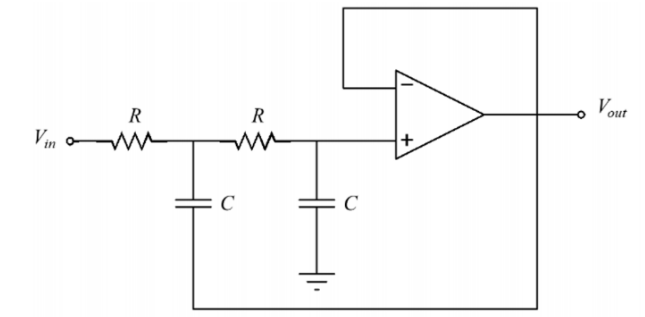
\includegraphics[width=0.8\textwidth]{images/2ndLow.png}
    \caption{Sallen-key low pass}
    \label{}
\end{figure}
\begin{equation}
    \begin{split}
        f_c = \frac{1}{2\pi\sqrt{R_1 R_2 C_1 C_2}}\\
    \end{split}
\end{equation}

\begin{figure}[h]
    \centering
    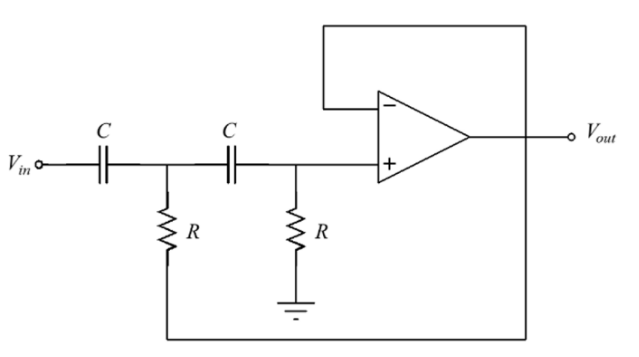
\includegraphics[width=0.8\textwidth]{images/2ndHigh.png}
    \caption{Sallen-key high pass}
    \label{}
\end{figure}
\begin{equation}
    f_c = \frac{1}{2\pi\sqrt{R_1R_2C_1C_2}}
\end{equation}